\section{Dataset and Evaluation Details}

\subsection{Dataset Construction and Documentation Checklist}
\label{sec:appendix:dataset_documentation}

The available study workflow establishes the high-level sequence used to construct
APT-Bench: clinical peripheral-blood specimens from five cancer groups and healthy
controls are converted to single-cell suspensions; cell-profile and viability quality
control precedes a paired single-cell transcriptome and 293-aptamer assay; separate
transcriptome and aptamer-barcode libraries are linked at the cell level; and
transcriptome-derived clusters and annotations provide the cell labels. For a
benchmark release, this overview must be accompanied by the following provenance
and protocol fields.

\paragraph{Outstanding disease-confounding validation.}
\todo{Obtain a sample-linked acquisition manifest from the data owner: patient
and sample IDs, collection and processing dates, APT assay batch, plate/pool,
reagent lot, library-preparation batch, sequencing run, site, and available
fresh/frozen and handling records. Audit disease-by-batch overlap before
choosing a validation design. Where disease groups have adequate cross-batch
support, evaluate patient-disjoint, held-out-batch generalization with all
preprocessing and selection restricted to training data. If disease and batch
are inseparable, obtain crossed-batch samples or an independent APT cohort;
statistical adjustment alone cannot identify their separate contributions.
The NC matrices must not be treated as external validation if they are the
healthy subset of this cohort. These validations are pending, not completed.}
Expression and QC matrices alone do not establish acquisition provenance;
archived disease analyses cannot establish disease-specific biological effects.

\paragraph{Transcriptomic preprocessing and cell quality control.}
The transcriptomic count matrix was processed with Seurat following its standard
workflow of normalization, feature selection, dimensionality reduction,
neighborhood-graph construction, and clustering \citep{hao2021integrated}.
DoubletFinder was used to identify and remove predicted doublets
\citep{mcginnis2019doubletfinder}. Low-quality cells were additionally filtered
using per-cell UMI count, detected-gene count, and mitochondrial-transcript
fraction. These steps preceded cluster annotation and construction of the linked
APT benchmark cohort. \todo{Report the Seurat and DoubletFinder versions, every
parameter and random seed, the exact UMI/gene/mitochondrial thresholds, and cell
counts before and after each filter.}

\paragraph{Manual annotation and reference-label reliability.}
After Seurat clustering, investigators manually assigned lineage and subtype
names by inspecting canonical marker-gene expression reported in prior PBMC and
pan-cancer studies \citep{zhang2024pan,yang2024pan}. No quantitative annotation
confidence, inter-annotator agreement, or external reference-transfer score is
available. Accordingly, these labels are operational reference annotations, not
error-free biological ground truth, and benchmark scores are conditional on this
manual taxonomy. The \emph{Unknown} label was assigned when a cluster did not show
a coherent canonical marker pattern for the expected PBMC subtypes; this was a
manual reject decision rather than a calibrated confidence threshold. Unknown
cells are excluded from the primary 27-subtype benchmark. \todo{Provide the full
subtype-by-marker citation table, the number and expertise of annotators, whether
they were blinded to disease, the adjudication procedure, and the explicit rule
used to assign Unknown.}

\paragraph{Cross-disease semantics and hierarchy mapping.}
The same 27 subtype labels and definitions were applied across all six disease
groups; no subtype was renamed or redefined for a particular disease. This gives
the labels a consistent operational meaning, but it does not prove that marker
expression or biological state is invariant across diseases. Each subtype is
assigned to one of five parent lineages by a manually curated lookup.
The exported lookup and structural audit are available under
\texttt{benchmark/release\_audit/}: the existing subtype summary has 27 unique
subtypes, five parents, and 361{,}792 cells, and the fold manifest has five
disjoint groups of eight patients. These checks establish internal bookkeeping
consistency, not independent biological validity.
\todo{Document independent validation of the subtype-to-lineage mapping, including
reviewers, disagreements, adjudication, and any marker-based checks.}

\begin{itemize}
    \item \todo{Report recruiting site(s) and dates, prospective versus retrospective
    collection, exact patient count per group, inclusion/exclusion and diagnostic
    criteria, and whether each participant contributed exactly one specimen.}
    \item \todo{Report available demographics and clinical covariates, including age,
    sex, disease stage, treatment status, and comorbidities; summarize missingness and
    state which fields cannot be released.}
    \item \todo{Report blood volume, collection tubes, time to processing, cell-isolation
    and cryopreservation procedures, quality-control thresholds, and sample/cell
    exclusion counts.}
    \item \todo{Report assay/platform and reagent versions, sequencing instruments and
    depth, 293-probe panel design, and a verified protein-target manifest or explicitly
    state why only anonymized probe identifiers can be released.}
    \item \todo{Report barcode-matching rates, APT normalization and filtering,
    all remaining software versions and parameters, and whether annotation was
    performed before investigators examined APT profiles or disease labels.}
    \item The documented final cell-flow accounting is
    $374{,}854\ \text{linked post-QC cells}
    -13{,}062\ \text{Unknown cells}=361{,}792\ \text{benchmark cells}$.
    \todo{Data owners: provide participant and cell counts at all earlier
    collection/QC exclusions before a complete cohort-flow diagram can be
    drawn. Supply the approval, consent, access, and licensing evidence listed
    in the Ethics and Reproducibility Statements.}
\end{itemize}


\subsection{Benchmark Interface and Release Contract}
\label{sec:appendix:benchmark_release}

The cell-typing interface records pseudonymous cell and patient IDs, fixed
folds, feature IDs, reference and predicted labels, and ontology columns.
A complete release requires the processed paired matrices, permissions and
access procedure, reference configurations, and a raw-data-to-evaluator
command. The current split manifest, selected artifact checksums and rebuild
commands cover only part of that release.
\todo{Finalize anonymous data/code access, licenses, original training
environment locks, archival versioning, and the portable end-to-end command.
Where access is controlled, provide the complete schema and access procedure.}

\begin{table*}[t]
\centering
\small
\setlength{\tabcolsep}{6pt}
\textbf{(a) Task and evaluation scope}\\[3pt]
\begin{tabular}{llllc}
\toprule
Resource & Primary input & Reported scope & Main unit & Hierarchy \\
\midrule
Open Problems & Multiple & 12 living tasks & Task-specific & Task-specific \\
scMultiBench & RNA/ADT/ATAC & 64 real + 22 simulated & Cell/dataset & No \\
SPARE & scRNA-seq & 5 datasets, 8 methods & Sample & No \\
PaSCient & scRNA-seq & 12.5M cells, 2,700 patients & Patient & No \\
APT-Bench & 293 aptamers & 1 cohort, 40 patients & Cell + patient & Yes \\
\bottomrule
\end{tabular}
\vspace{6pt}

\textbf{(b) Protocol components and availability}\\[3pt]
\begin{tabular}{lcccc}
\toprule
Resource & Patient task & Two-axis scale & Assay budget & Public pipeline \\
\midrule
Open Problems & Task-specific & No & No & Yes \\
scMultiBench & No & No & Feature selection & Yes \\
SPARE & Yes & No & No & Yes \\
PaSCient & Yes & No & No & Not audited \\
APT-Bench & Secondary & Separate report & Secondary & Pending release \\
\bottomrule
\end{tabular}
\caption{Scope comparison with recent single-cell evaluation resources
\citep{luecken2025open,liu2025multitask,shitov2025spare,liu2026pascient}.
``Task-specific'' means that the living platform defines multiple contracts
rather than one shared clinical protocol. APT-Bench is narrower in cohorts but
centers a fixed aptamer modality and patient-disjoint coarse-to-fine cell
typing. Patient-level analysis is secondary; sampling studies are in a separate
report and do not expand the main contribution. Public release remains a submission requirement, not a completed
claim.}
\label{tab:benchmark_comparison}
\end{table*}


\subsection{Supporting Split-Protocol Audit}
\label{sec:results:protocol}

Cell-level splitting raises cell-weighted coarse/fine Macro-F1 by
0.050/0.069 for XGBoost and 0.090/0.108 for Soft-cascade
(Table~\ref{tab:protocol_sensitivity}). The apparent fine model difference
is 0.048 under cell splitting versus approximately 0.009 under
patient-disjoint evaluation. Training/test allocations also differ: this is
a protocol comparison, not a matched causal estimate of leakage or evidence
of universal ranking reversal. Neither column uses the subject-balanced
main-leaderboard metric.

\begin{table}[t]
\centering
\small
\setlength{\tabcolsep}{6pt}
\renewcommand{\arraystretch}{1.10}

\begin{tabular}{llccc}
\toprule
\textbf{Task} & \textbf{Model} & \textbf{Patient-level} & \textbf{Cell-level} & \textbf{Inflation} \\
\midrule

\multirow{2}{*}{Coarse lineage}
& XGBoost      & 0.322 & 0.372 & $+0.050$ \\
& \ourmethod{} & 0.333 & 0.432 & $+0.099$ \\
\midrule

\multirow{2}{*}{Fine subtype}
& XGBoost      & 0.143 & 0.212 & $+0.069$ \\
& \ourmethod{} & 0.156 & 0.261 & $+0.105$ \\

\bottomrule
\end{tabular}

\caption{
Macro-F1 under the primary patient-level 5-fold protocol versus the
cell-level protocol-sensitivity control (\S\ref{sec:data:protocols}), both
evaluated on the same models. Cell-level splitting, which allows cells from
the same patient to appear in both training and test sets, inflates
macro-F1 for both models, and inflates \ourmethod{}'s score by roughly
twice as much as XGBoost's. This indicates that \ourmethod{}'s
representation is more sensitive to patient-level leakage than a
tree-based baseline, underscoring why patient-independent evaluation is
necessary to avoid overstating hierarchical classification performance in
this small-cohort setting.
}
\label{tab:protocol_sensitivity}

\end{table}


\subsection{Hierarchy and Conditional-Pairing Diagnostic Protocol}
\label{sec:appendix:identity_questions}

This exploratory follow-up was specified after inspecting the original
single-seed results, not preregistered. Its frozen implementation is
\texttt{analysis/cell\_identity\_questions.py}; the associated protocol
\texttt{CELL\_IDENTITY\_QUESTIONS\_V1.md} records the full specification.

\paragraph{Completed full-budget hierarchy control.}
The three-seed MLP uses every development cell in five patient-disjoint
folds. Conditional priors use only actual outer-refit subtype counts:
majority decoding and an expected-confusion baseline, not expected
finite-sample F1. Oracle decoding masks scores to the true parent's children.
Within each lineage, eligible patients' confusion matrices are normalized
before pooling and macro-averaging fixed child classes. Zero-support patients
are excluded and counted; outside-lineage predictions retain false negatives.

\paragraph{Matched-input follow-up (running).}
SGD and MLP retain the existing folds, 1{,}000-cell-per-training-patient cap,
40 epochs, and inner-patient selection over their two-value regularization
grids. Three training seeds each have three patient-shuffle and three
patient-by-lineage-shuffle draws. RNA, APT, paired RNA+APT, and RNA+noise
use the same selection rule. Whole APT vectors move only within the
specified group, separately in train and evaluation partitions; singleton
and unchanged-pair fractions are recorded. True test lineage is privileged,
not deployable input. Oracle replays must exactly reconstruct stored
ordinary predictions before acceptance.

\paragraph{RNA difficulty and uncertainty.}
The inner-validation 20th-percentile RNA probability-margin threshold is
frozen for outer testing. All cells, every lineage, low-margin cells, and
retrospective RNA-error/correct strata are reported with identical cells
and class columns across controls. Error/correct strata jointly show rescue
and damage, not independent validation. Scores are subject-balanced pooled
Macro-F1 and mean within-scope patient accuracy. Joint resampling of training
seeds, shuffles within seed, and paired patients gives 2{,}000 pointwise
95\% intervals, not multiplicity-adjusted confirmation; three seeds provide
limited training-uncertainty evidence.

\paragraph{RNA representation sensitivity.}
HVG selection and normalization use training partitions only. Beyond the
2{,}000-HVG probe, the existing 5{,}000-HVG reference grid is retained
regardless of outcome. Targeted 5{,}000-HVG conditional shuffling is triggered
if MLP paired-minus-RNA and paired-minus-patient-by-lineage-shuffle effects
are positive in all three seeds and both joint intervals exclude zero.
SGD and all negative contrasts remain reported. This computational gate is
not robustness evidence; an increment can still depend on restricted RNA
representation rather than uniquely aptamer-specific biology.


\subsection{Full-Budget Hierarchy Support}
\label{sec:appendix:full_budget_hierarchy}

The full-budget 256/128-unit MLP uses all development cells and a different
optimization recipe from the capped 64-unit matched-input MLP. Its overall
ordinary/oracle/expected-prior scores are 0.141/0.385/0.180.
The oracle-minus-prior difference is $+0.205$ ($[0.174,0.217]$).
Figure~\ref{fig:lineage_structure} reports every lineage. Differences from the
matched-input experiment cannot be attributed to training-cell budget alone,
because architecture, optimization and selection also differ.

\begin{figure}[H]
\centering
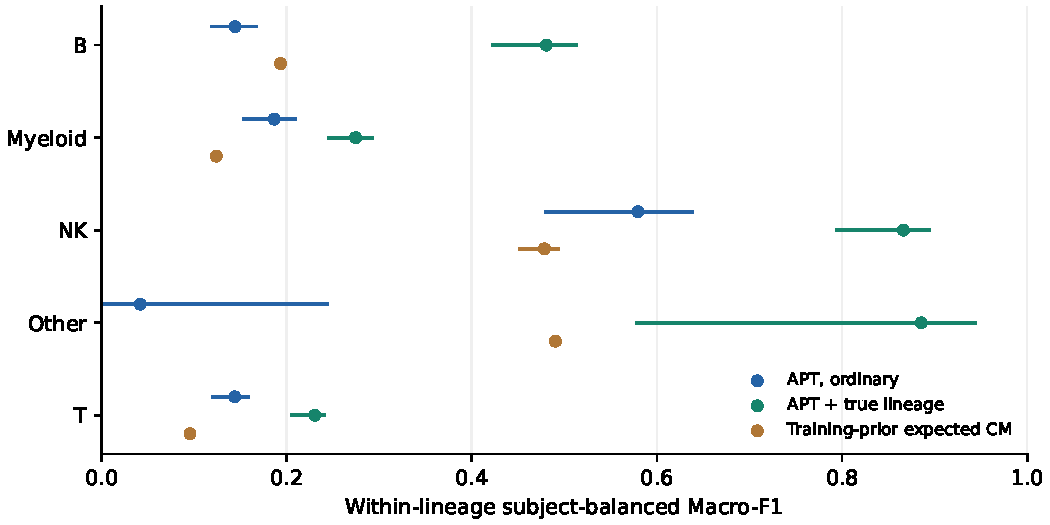
\includegraphics[width=\linewidth]{outputs/cell_identity_questions_v1/full_mlp_lineages/lineage_structure.pdf}
\caption{Full-budget MLP support: three-seed means and pointwise joint
seed/patient 95\% intervals. Each eligible patient's matrix is normalized
within the displayed lineage, then pooled before Macro-F1 is computed over
its fixed children. Outside-lineage predictions remain false negatives.
These scores cannot be averaged across lineages to reconstruct Table~\ref{tab:main}.
The conditional-proportion baseline is F1 of an expected confusion matrix,
not expected F1. Oracle information is privileged. This is not the capped-budget
APT--RNA comparison in Figure~\ref{fig:matched_lineage_identity}.}
\label{fig:lineage_structure}
\end{figure}

\subsection{True-Lineage Restricted Decoding}
\label{sec:appendix:true_lineage_oracle}

We replay the 15 frozen final checkpoints (three neural references, five
patient-disjoint folds), retain explicit cell IDs and ontology columns,
and require exact reconstruction of their original coarse and fine predictions
before computing this diagnostic. For each of the same 361{,}792 held-out cells,
we mask the fine score vector to subtypes whose parent is the true lineage,
then take its argmax. We do not change Soft-cascade routing or condition the
evaluation set on a correct coarse prediction. The diagnostic therefore uses
privileged test-label information and cannot be placed on the deployable
leaderboard. Table~\ref{tab:true_lineage_oracle} reports subject-balanced pooled
Macro-F1 and paired patient-bootstrap differences, conditional on these frozen
models. Reduced candidate-set size contributes to the gain; neither the gain
nor the remaining error identifies an assay-specific information ceiling.

\begin{table}[htbp]
\centering\small
\setlength{\tabcolsep}{5pt}
\begin{tabular}{lccc}
\toprule
Model & Ordinary fine & True-lineage oracle & Paired gain [95\% CI] \\
\midrule
Flat Transformer & 0.139 & 0.366 & +0.227 [0.202, 0.238] \\
HCE Transformer & 0.143 & 0.361 & +0.218 [0.196, 0.231] \\
Soft-cascade Transformer & 0.145 & 0.358 & +0.214 [0.194, 0.230] \\
\bottomrule
\end{tabular}
\caption{Privileged true-lineage restricted decoding on the same frozen
predictions. Scores are subject-balanced pooled Macro-F1; gains use 2{,}000
paired patient-bootstrap resamples and pointwise intervals, conditional on
fitted models. The oracle knows the true parent and is not a deployable method.}
\label{tab:true_lineage_oracle}
\end{table}



\subsection{Complete Per-Subtype Reporting}
\label{sec:appendix:subtype_audit}

Table~\ref{tab:subtype_per_class} retains all 27 subtypes, cell counts,
patient coverage, and historical cell-weighted per-class F1 with 2,000
patient-bootstrap intervals. These are not the subject-balanced main metric.
They support transparent class-level inspection, not a biological
interpretation of marginal support--performance correlations.
\begingroup
\scriptsize
\setlength{\tabcolsep}{3.2pt}
\renewcommand{\arraystretch}{1.04}
\begin{longtable}{llrrrrrr}
\caption{Per-subtype support and pooled out-of-fold F1 with 95\% percentile intervals from 2{,}000 patient-clustered bootstrap resamples. Cells/patient is the mean among patients in which that subtype is observed. Head and Tail denote the seven most and seven least abundant subtypes; all others are Mid.}\label{tab:subtype_per_class} \\
\toprule
\textbf{Subtype} & \textbf{Lineage} & \textbf{Cells} & \textbf{Patients} & \textbf{Cells/patient} & \textbf{Regime} & \textbf{DropCascade F1 [95\% CI]} & \textbf{XGB F1 [95\% CI]} \\
\midrule
\endfirsthead
\toprule
\textbf{Subtype} & \textbf{Lineage} & \textbf{Cells} & \textbf{Patients} & \textbf{Cells/patient} & \textbf{Regime} & \textbf{DropCascade F1 [95\% CI]} & \textbf{XGB F1 [95\% CI]} \\
\midrule
\endhead
\midrule
\multicolumn{8}{r}{Continued on next page} \\
\endfoot
\bottomrule
\endlastfoot
Erythrocyte & Other & 65 & 6 & 10.8 & Tail & 0.253 [0.000, 0.395] & 0.133 [0.000, 0.545] \\
Atypical Memory B & B & 781 & 34 & 23.0 & Tail & 0.005 [0.000, 0.014] & 0.005 [0.000, 0.014] \\
CD4 Monocyte-4 & Myeloid & 1,405 & 35 & 40.1 & Tail & 0.027 [0.006, 0.053] & 0.014 [0.000, 0.033] \\
platelet & Other & 1,574 & 38 & 41.4 & Tail & 0.078 [0.016, 0.125] & 0.063 [0.015, 0.106] \\
Tcm & T & 2,121 & 36 & 58.9 & Tail & 0.000 [0.000, 0.000] & 0.004 [0.000, 0.016] \\
Memory B-2 & B & 2,130 & 33 & 64.5 & Tail & 0.017 [0.004, 0.033] & 0.011 [0.000, 0.024] \\
Plasma & B & 2,173 & 40 & 54.3 & Tail & 0.611 [0.522, 0.684] & 0.599 [0.496, 0.685] \\
pDC & Myeloid & 2,615 & 40 & 65.4 & Mid & 0.029 [0.010, 0.061] & 0.019 [0.005, 0.040] \\
CD14 Monocyte-3 & Myeloid & 2,977 & 32 & 93.0 & Mid & 0.258 [0.170, 0.306] & 0.177 [0.103, 0.211] \\
CD8 + CTL-3 & T & 3,244 & 27 & 120.1 & Mid & 0.020 [0.004, 0.035] & 0.023 [0.008, 0.043] \\
GCB & B & 3,283 & 31 & 105.9 & Mid & 0.039 [0.007, 0.071] & 0.047 [0.001, 0.073] \\
Cycling T & T & 3,667 & 40 & 91.7 & Mid & 0.028 [0.015, 0.043] & 0.012 [0.003, 0.022] \\
CD14 Monocyte-2 & Myeloid & 3,931 & 40 & 98.3 & Mid & 0.075 [0.046, 0.102] & 0.078 [0.056, 0.097] \\
CD8 + CTL-2 & T & 4,049 & 33 & 122.7 & Mid & 0.069 [0.017, 0.116] & 0.078 [0.015, 0.113] \\
CD16 Monocyte-2 & Myeloid & 5,142 & 40 & 128.6 & Mid & 0.111 [0.064, 0.161] & 0.117 [0.063, 0.164] \\
CD8 + CTL-1 & T & 7,303 & 40 & 182.6 & Mid & 0.009 [0.000, 0.024] & 0.002 [0.001, 0.004] \\
cDC2 & Myeloid & 7,376 & 40 & 184.4 & Mid & 0.132 [0.099, 0.181] & 0.125 [0.079, 0.167] \\
CD8 Tem-2 & T & 10,548 & 40 & 263.7 & Mid & 0.019 [0.005, 0.038] & 0.017 [0.008, 0.030] \\
CD16 Monocyte-1 & Myeloid & 14,678 & 40 & 366.9 & Mid & 0.152 [0.111, 0.198] & 0.118 [0.090, 0.150] \\
CD4 + Tcm-2 & T & 16,861 & 39 & 432.3 & Mid & 0.188 [0.111, 0.236] & 0.188 [0.136, 0.220] \\
Naive T & T & 17,960 & 40 & 449.0 & Head & 0.131 [0.067, 0.183] & 0.149 [0.073, 0.199] \\
Memory B-1 & B & 23,722 & 40 & 593.0 & Head & 0.034 [0.020, 0.048] & 0.032 [0.017, 0.047] \\
CD8 Tem-1 & T & 26,714 & 40 & 667.9 & Head & 0.187 [0.128, 0.250] & 0.162 [0.107, 0.221] \\
CD14 Monocyte-1 & Myeloid & 29,871 & 40 & 746.8 & Head & 0.437 [0.378, 0.495] & 0.451 [0.392, 0.507] \\
CD56 NK & NK & 38,442 & 40 & 961.0 & Head & 0.398 [0.320, 0.436] & 0.437 [0.373, 0.480] \\
CD16 NK & NK & 58,507 & 40 & 1462.7 & Head & 0.383 [0.326, 0.434] & 0.376 [0.317, 0.429] \\
CD4 + Tcm-1 & T & 70,653 & 40 & 1766.3 & Head & 0.417 [0.368, 0.460] & 0.435 [0.393, 0.473] \\
\end{longtable}
\endgroup


\subsection{Scoring Units and Supporting Split Comparison}
\label{sec:appendix:protocol_sensitivity}
\label{sec:results:protocol}

\paragraph{Metric definitions.}
Let $C^{(p)}\in\mathbb{R}^{K\times K}$ be the confusion matrix for held-out
subject $p$ and $n_p=\sum_{ij}C^{(p)}_{ij}$. We distinguish
\begin{align}
C^{\mathrm{CW}} &= \sum_p C^{(p)},
&F_1^{\mathrm{CW}} &= \operatorname{MacroF1}(C^{\mathrm{CW}}),\\
C^{\mathrm{SB}} &= \frac{1}{P}\sum_p\frac{C^{(p)}}{n_p},
&F_1^{\mathrm{SB}} &= \operatorname{MacroF1}(C^{\mathrm{SB}}),\\
F_1^{\mathrm{within}} &= \frac{1}{P}\sum_p
\operatorname{MacroF1}(C^{(p)}). &&
\end{align}
We call these \emph{cell-weighted pooled Macro-F1}, \emph{subject-balanced
pooled Macro-F1}, and \emph{mean within-subject Macro-F1}. Subject balancing
normalizes each subject confusion matrix to unit mass before pooling; it is
neither equal-cell subsampling nor averaging per-subject Macro-F1. Released
files retain the legacy column name \texttt{patient\_balanced\_macro\_f1} for
$F_1^{\mathrm{SB}}$, but no different patient-balanced statistic is used.

The numerical split comparison appears in this appendix
(Table~\ref{tab:protocol_sensitivity}). Its historical scores are cell-weighted
in both columns, rather than the subject-balanced leaderboard metric.

Exact subject-normalized pooling is primary. The older equal-cell Monte
Carlo sensitivity remains archived, rather than occupying a separate table.


Cell-level splitting raises cell-weighted coarse/fine Macro-F1 by
0.050/0.069 for XGBoost and 0.090/0.108 for Soft-cascade.
Training/test allocations also differ: this is a descriptive protocol
comparison rather than an isolated causal estimate of leakage.
\begin{table}[t]
\centering
\small
\setlength{\tabcolsep}{6pt}
\renewcommand{\arraystretch}{1.10}

\begin{tabular}{llccc}
\toprule
\textbf{Task} & \textbf{Model} & \textbf{Patient-level} & \textbf{Cell-level} & \textbf{Inflation} \\
\midrule

\multirow{2}{*}{Coarse lineage}
& XGBoost      & 0.322 & 0.372 & $+0.050$ \\
& \ourmethod{} & 0.333 & 0.432 & $+0.099$ \\
\midrule

\multirow{2}{*}{Fine subtype}
& XGBoost      & 0.143 & 0.212 & $+0.069$ \\
& \ourmethod{} & 0.156 & 0.261 & $+0.105$ \\

\bottomrule
\end{tabular}

\caption{
Macro-F1 under the primary patient-level 5-fold protocol versus the
cell-level protocol-sensitivity control (\S\ref{sec:data:protocols}), both
evaluated on the same models. Cell-level splitting, which allows cells from
the same patient to appear in both training and test sets, inflates
macro-F1 for both models, and inflates \ourmethod{}'s score by roughly
twice as much as XGBoost's. This indicates that \ourmethod{}'s
representation is more sensitive to patient-level leakage than a
tree-based baseline, underscoring why patient-independent evaluation is
necessary to avoid overstating hierarchical classification performance in
this small-cohort setting.
}
\label{tab:protocol_sensitivity}

\end{table}


\subsection{Additional Reference Inventory}
\label{sec:appendix:consistency}

Table~\ref{tab:hierarchy_sb_all} includes auxiliary classical references and
the full-budget MLP. Interval types are labeled as in the main table.
Historical cell-weighted leaderboards, auxiliary path metrics and their
original testing family are retained in the versioned source archive, not
duplicated as another primary comparison.
\begin{table}[H]
\centering\small
\setlength{\tabcolsep}{6pt}
\begin{tabular}{llcc}
\toprule
Model & CI & Coarse SB-Macro-F1 $\uparrow$ & Fine SB-Macro-F1 $\uparrow$ \\
\midrule
Linear SVM & P & 0.309 [0.292, 0.324] & 0.105 [0.089, 0.118] \\
Random Forest & P & 0.253 [0.227, 0.277] & 0.089 [0.079, 0.097] \\
Reference Correlation & P & 0.171 [0.147, 0.192] & 0.068 [0.050, 0.078] \\
\bottomrule
\end{tabular}
\caption{Additional APT-only references, complementing Table~\ref{tab:main}.
P denotes pointwise 95\% patient-bootstrap intervals conditional on frozen fits.}
\label{tab:hierarchy_sb_all}
\end{table}


\subsection{Patient Composition Recovery}
\label{sec:appendix:composition_recovery}
For each of the 40 outer-test patients, we compare the mean soft cell-type
probabilities with reference cell fractions. The constant baseline is the
equal-patient mean reference composition of the 32 outer-development patients
in that fold; no test-patient annotations enter its construction. For $K$
classes and $N$ test patients, the recovery error is
\[
 E=\frac{1}{N}\sum_{p=1}^{N}\frac{1}{K}\sum_{k=1}^{K}
 |\widehat{\pi}_{pk}-\pi_{pk}|.
\]
We report $E_{\mathrm{baseline}}-E_{\mathrm{model}}$, so positive values favor
predicted compositions. All five lineages or all 27 subtypes are included,
without selecting well-recovered classes. Absolute errors across these two
resolutions are not directly comparable because their denominators differ.
Using 2,000 disease-stratified paired patient-bootstrap replicates, subtype
error decreases from 0.02314 to 0.01478, a reduction of 0.00836
($[0.00648,0.01010]$). Lineage error changes from 0.05495 to 0.05827, a
reduction of $-0.00332$ ($[-0.01389,0.00670]$). Intervals are pointwise and
conditional on the completed cross-fitted cell models; they do not include
training-subset or model-fitting uncertainty. The accompanying per-class
audit reports error, signed bias, and rank correlation for every class.
Disease-adjusted rank correlations residualize both ranked fractions on
disease-group indicators and are descriptive, not evidence of biological
specificity or causal independence from disease. Reference recovery does not
validate the annotation itself or imply improved disease characterization.

\paragraph{Total variation and direct regression.}
For probability vectors, $\mathrm{TV}(\widehat\pi,\pi)=
\tfrac12\sum_k|\widehat\pi_k-\pi_k|$, so mean TV is exactly $KE/2$.
For subtypes, baseline/model mean TV is 0.312/0.200; this is the same
information as MAE, not a second validation endpoint. Per-class bias and
centered recovery errors include every class, including rare subtypes.

We additionally fit patient-median APT directly to reference composition using
multioutput ridge regression. Each outer fold uses the remaining four frozen
patient folds to select $\alpha\in\{0.1,1,10,100,1000\}$ by MAE after
Euclidean projection onto the probability simplex. Standardization is fitted
within each training split. This control uses provided APT expression values,
not a newly selected normalization, and no disease labels enter fitting.
Table~\ref{tab:direct_composition} reports all three methods. The soft-minus-direct
subtype MAE difference is $+0.00057$ ($[-0.00092,0.00211]$), so there is no
resolved advantage of cell-output aggregation over direct regression.
Intervals use 2,000 disease-stratified paired patient draws with seed
20260912. Full per-class MAE, bias, and centered-error outputs are
provided with the analysis, without selecting favorable classes.
\begin{table}[t]
\centering\small
\begin{tabular}{lrrrr}
\toprule
& \multicolumn{2}{c}{Lineage} & \multicolumn{2}{c}{Subtype} \\
Method & MAE & TV & MAE & TV \\
\midrule
Training-patient mean & 0.05495 & 0.137 & 0.02314 & 0.312 \\
Soft cell-output mean & 0.05827 & 0.146 & 0.01478 & 0.200 \\
Median APT ridge & 0.05324 & 0.133 & 0.01421 & 0.192 \\
\bottomrule
\end{tabular}
\caption{Patient-composition recovery on the same 40 outer-test patients.
Lower is better. Mean TV equals $K\,\mathrm{MAE}/2$ and is not independent
evidence. Direct regression uses inner-selected ridge and simplex projection;
soft composition uses frozen nested XGBoost predictions. Soft-minus-direct
MAE differences are $+0.00503$ ($[-0.00415,0.01469]$) for lineage and
$+0.00057$ ($[-0.00092,0.00211]$) for subtype (pointwise paired 95\%
patient-bootstrap intervals). Neither contrast establishes equivalence.}
\label{tab:direct_composition}
\end{table}



\subsection{Archived Analyses}
\label{sec:appendix:minimal_panel}
\label{sec:appendix:sampler}

The original single-seed paired-input pilot, chance adjustment, disease
classification audits, marginal support correlations and redundant
cell-weighted metrics are retained in the source archive and their analysis
outputs. They are not additional evidence for the present two cell-identity
findings. Disease-classification point estimates are not reported in this
manuscript; acquisition validation remains outstanding in the dataset
documentation. The archive index records the old sections and their replacements.

\subsection{Exploratory Leave-One-Disease-Out Stress Test}
\label{sec:appendix:novelty}

For each leave-one-disease-out (LODO) run, all patients from one group are
withheld from training. The available table contains five cancer-group
summaries. A numerical Normal-held-out artifact and row-level support counts
have not been verified, so the sixth row is explicitly unavailable rather
than omitted. These cell-weighted group summaries are not averaged or
subtracted from pooled five-fold scores, since their evaluation populations
and training protocols differ. This is an incomplete descriptive stress test;
cross-disease generalization requires external, patient-clustered validation.
Unmatched detector rankings are omitted.

\begin{table}[t]
\centering
\small
\setlength{\tabcolsep}{4pt}
\renewcommand{\arraystretch}{1.10}

\resizebox{\columnwidth}{!}{
\begin{tabular}{lccccc}
\toprule
\textbf{Held-out Disease}
& \textbf{Fine Macro-F1}
& \textbf{Fine Acc.}
& \textbf{Coarse Macro-F1}
& \textbf{Coarse Acc.}
& \textbf{Tail Macro-F1} \\
\midrule
BTC
& 0.086 & 0.317 & 0.310 & 0.479 & 0.073 \\
CRC
& 0.105 & 0.277 & 0.309 & 0.520 & 0.112 \\
GC
& 0.063 & 0.269 & 0.281 & 0.488 & 0.057 \\
HCC
& 0.063 & 0.246 & 0.264 & 0.383 & 0.072 \\
PC
& 0.057 & 0.253 & 0.221 & 0.482 & 0.037 \\
\midrule
\textbf{Macro-average}
& \textbf{0.075}
& \textbf{0.272}
& \textbf{0.277}
& \textbf{0.470}
& \textbf{0.070} \\
\bottomrule
\end{tabular}
}

\caption{
Leave-one-disease-out generalization for \ourmethod{} over the five
malignant held-out diseases. Each row withholds all patients of the named
disease from training. The in-distribution reference using the same model
under the standard patient-disjoint 5-fold protocol is fine Macro-F1
0.156 and coarse Macro-F1 0.333. A separate Normal-held-out run produces
near-chance fine performance and is discussed in the text as additional
evidence that unseen-disease transfer is difficult. LODO is reported here
as motivation for explicit novelty detection, not as proof that the model
already solves cross-disease generalization.
}
\label{tab:lodo}

\end{table}

